\section{wow}

\begin{figure}[htb!]
    \centering
    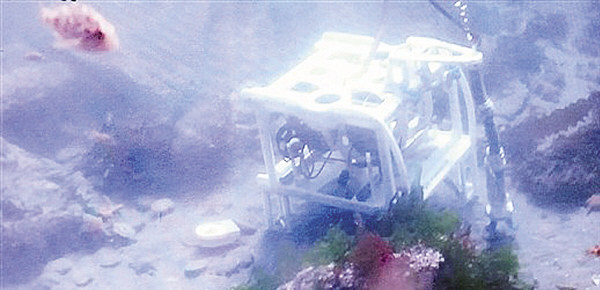
\includegraphics[width=0.9\textheight, angle=-90]{Figures/wow.jpg}
\end{figure}

\pagebreak

\section{Hardware and Software Configurations Used for Computer Vision}\label{a:cvconfig}

\begin{table}[ht]
    \renewcommand*{\arraystretch}{1.6}
    \centering
    \begin{tabularx}{\textwidth}{Xl}
        \multicolumn{2}{c}{\Large{Main Configuration of \citetitle{jetson} Used}}   \\
        \toprule
        \textbf{GPU}                & 512-core Volta GPU with Tensor Cores          \\
        \midrule
        \textbf{CPU}                & 8-core ARM v8.2 64-bit CPU, 8MB L2 + 4MB L3   \\
        \midrule
        \textbf{Memory}             & 32GB 256-Bit LPDDR4x | 137GB/s                \\
        \midrule
        \textbf{Storage}            & 32GB eMMC 5.1                                 \\
        \midrule
        \textbf{DL Accelerator}     & (2x) NVDLA Engines                            \\
        \midrule
        \textbf{Vision Accelerator} & 7-way VLIW Vision Processor                   \\
        \midrule
        \textbf{Encoder/Decoder}    & (2x) 4Kp60 | HEVC/(2x) 4Kp60 | 12-Bit Support \\
        \midrule
        \textbf{Size}               & 105 mm x 105 mm x 65 mm                       \\
        \midrule
        \textbf{Deployment}         & Module (Jetson AGX Xavier)                    \\
        \bottomrule
    \end{tabularx}
    \caption[Main Configuration of Jetson AGX Xavier Used]{}
\end{table}

\begin{table}[h]
    \renewcommand*{\arraystretch}{1.6}
    \centering
    \begin{tabularx}{\textwidth}{Xl}
        \multicolumn{2}{c}{\Large{Version of Libraries Used}} \\
        \toprule
        CUDA    & 10.0                                        \\
        \midrule
        cuDNN   & 7.6.5                                       \\
        \midrule
        OpenCV  & 3.4.11 (with GTK)                           \\
        \midrule
        PyTorch & 1.1.0 (LibTorch)                            \\
        \midrule
        ArUco   & 3.1.12                                      \\
        \bottomrule
    \end{tabularx}
    \caption[Version of Libraries Used]{}
\end{table}